\chapter{The multistream flow field in one-dimension}
\label{appendix:nstream}

\begin{figure}
\begin{minipage}[t]{.99\linewidth}
  \centering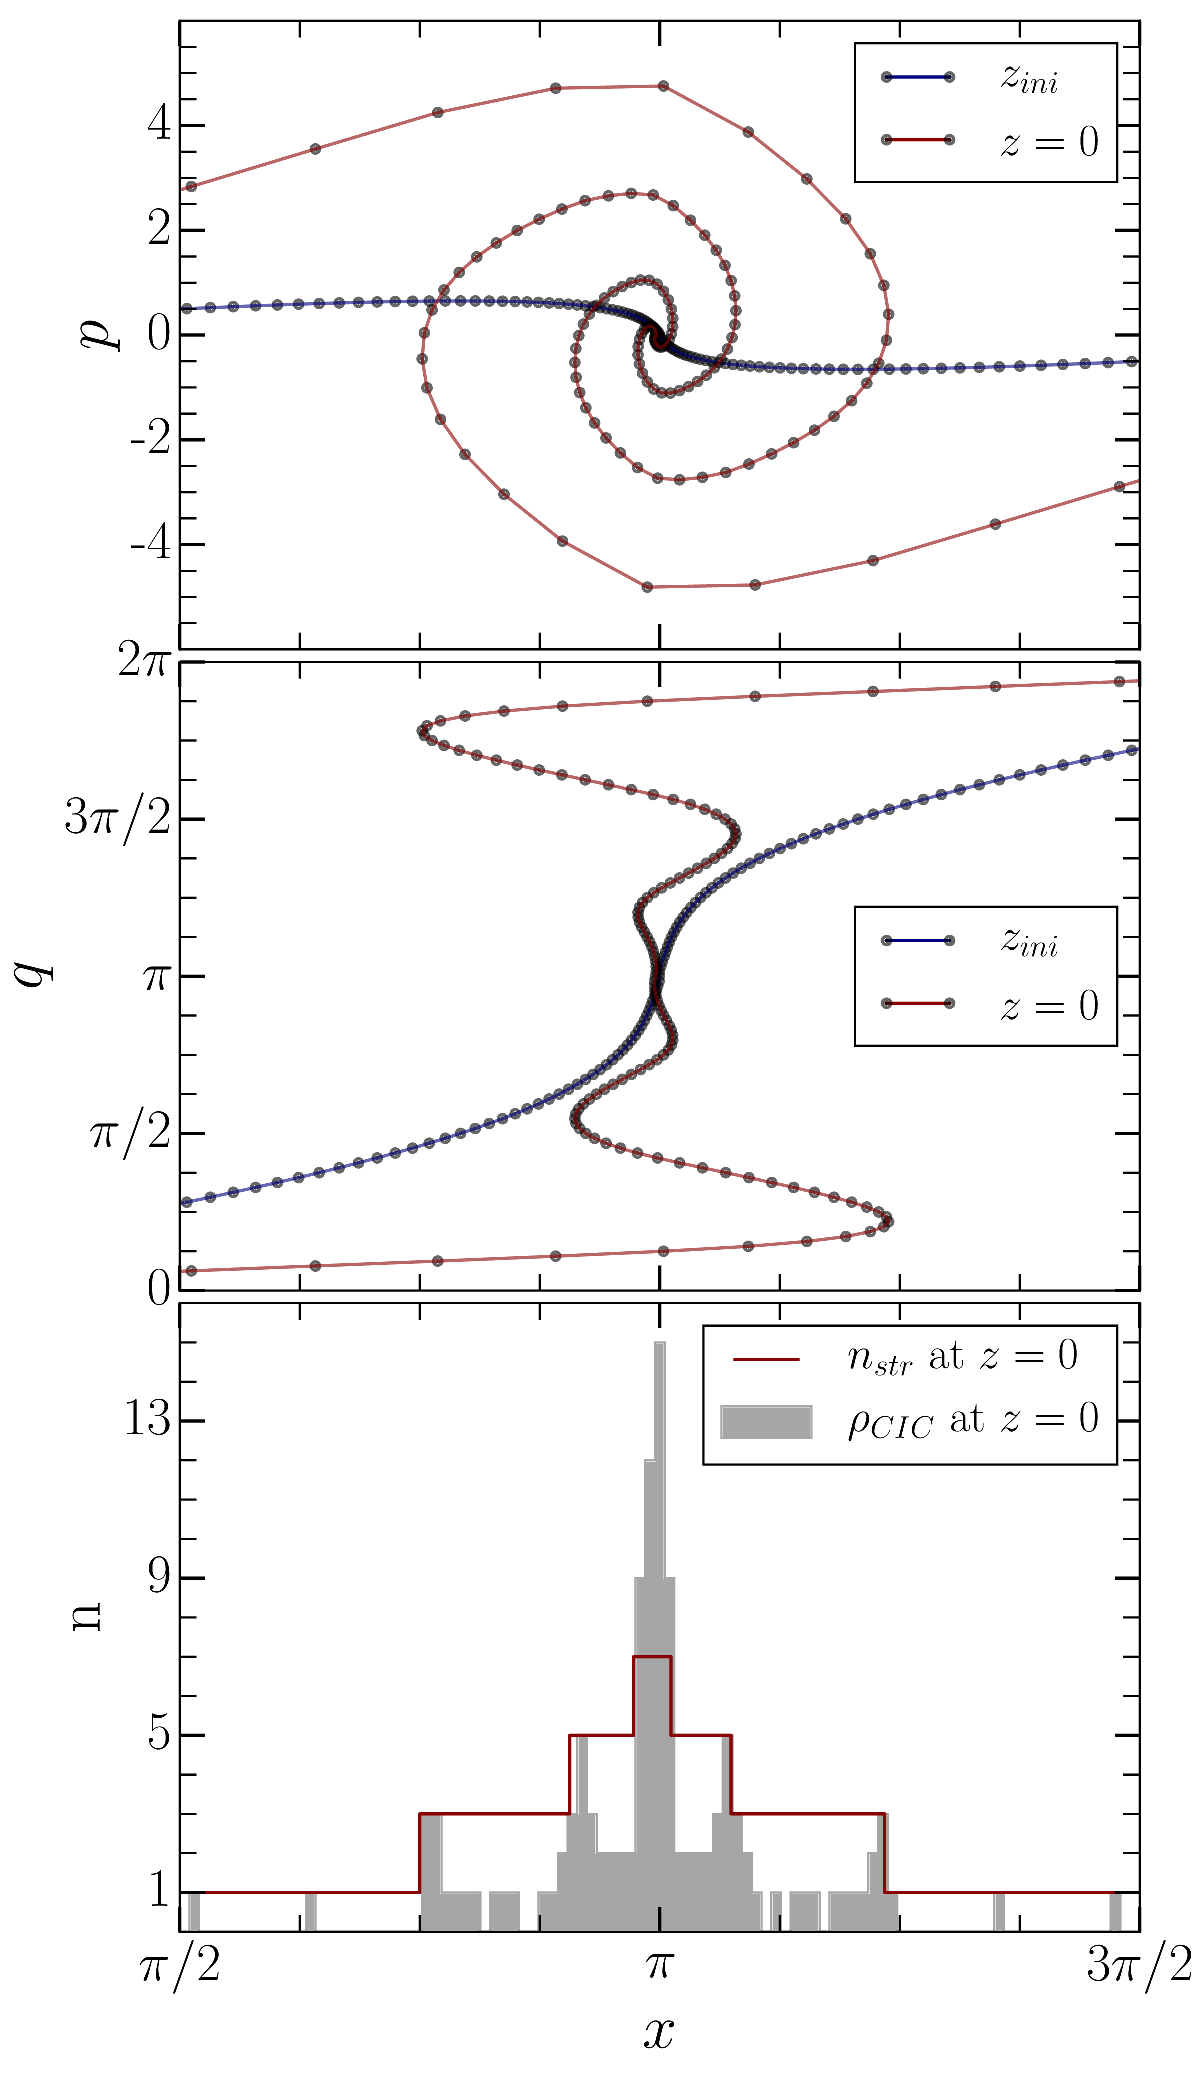
\includegraphics[width=8.cm]{Chapter4/Source_v2/fig13.pdf} 
\end{minipage}\hfill
\caption{ Multi-streaming in one-dimension gravitational collapse. Top panel: $(\bf{p}, \bf{x})$ phase-space representation redshift $z_{ini}$ and $z = 0$. Dots represent the dark matter particles. Initially the mass particles are in the linear stage of evolution. At $z = 0$, multiple values of $\bf{p}(\bf{x})$ is seen in the collapsed regions. Middle panel: Equivalent Lagrangian sub-manifold $\bf{q}(\bf{x})$. At $z_{ini}$, the dashed line represents $\bf{q} = \bf{x}$. Number of streams are parametrized from this sub-manifold. Bottom panel: The multistream field $n_{str}$ and the number-density using CIC algorithm, $n_{CIC}$ at $z = 0$. }
\label{fig:phase1d}
\end{figure}

The top panel in \autoref{fig:phase1d} shows the velocity multistreaming phenomenon in a one-dimensional collapse. The phase-space $(\bf{p}, \bf{x})$ (where $p$ is the momentum and $x$ is the co-moving Eulerian coordinate) is single-valued in the linear stage of evolution (at redshift $z_{ini}$). Non-linear stage of gravitational evolution of the collision-less dark matter particles then results in multi-valued $\bf{p} (\bf{x},z)$ at $z = 0$. The mass particles are sparsely  distributed outside the region of gravitational collapse, and are denser in the inner streams.

 
A dynamically equivalent transformation $(\bf{p}, \bf{x}) \mapsto (\bf{q}, \bf{x}) $ (where $\bf{q}$ is the Lagrangian coordinate) shows the Lagrangian sub-manifold in the middle panel of \autoref{fig:phase1d}. This two-dimensional phase-space has foldings that correspond to multiple velocity streams, although the sub-manifold itself remains continuous. A projection of the Lagrangian sub-manifold at each point in the configuration space quantifies the number-of-streams. Folding in the sub-manifold are checked for points in configuration space using tessellations. The tessellating simplices in one-dimensional model are just the line-segments whose nodes are the dark matter particles in the Lagrangian space. Dynamical property is accounted for in this phase-space tessellation since labels of the nodes remain intact throughout the evolution; the line segments may shorten, extend or change orientation. Each folding in the Lagrangian sub-manifold increases the number of streams by a factor of two. In three-dimensional simulations, the sub-manifold twists in complicated ways in a six-dimensional phase space. The number-of-streams in N-body simulations (\citealt{Shandarin2012} and \citealt{Abel2012b}) is calculated using Lagrangian/phase-space tessellations. This triangulation is conceptually different from the Voronoi (See \citealt{Schaap2000} and references therein) or Delaunay \citep{Icke1991} tessellation schemes. 

The bottom panel \autoref{fig:phase1d} shows the the multistream field $n_{str}(\bf{x})$ at $z = 0$. The field only takes the values of 1, 3, 5 and 7 in this scenario. Caustics occur at the folds in Lagrangian sub-manifold, and have a measure zero (study of caustics in one- and  two-dimensional evolution is done in \cite{Hidding2014}, three-dimensional caustic surface in a cosmological simulation is shown in \autoref{fig:NstrCaust}). Several properties of the multistream field are significantly different from mass density. The bottom panel also shows an illustration of CIC algorithm (cf. \citealt{Hockney1988}) in calculating density, which is numerically equivalent to counting the number of particles on each cell of a regular grid. One major difference is in the regions before gravitational collapse: $n_{str}$ is universally equal to unity, whereas number density fluctuates. It should also be noted that density by definition is a continuous field; numerical approximations like CIC discretise the field. Alternatively, multistream field is intrinsically a discrete-data field.  


\section{Variations in the multistream field}
\label{appendix:Eigen}

A second-order local variations of a scalar field $f$ is described by a Hessian. In a three-dimensional domain, the Hessian is given by \autoref{eq:Hess}. The geometry of the scalar field is classified by the Eigenvalues of the Hessian. The convex regions have at-most one maxima within the (3+1)-dimensional functional space. Projection of this closed region onto three-dimensional coordinate space also gives a closed surface in coordinate space. 


% An illustration of the projection is shown in \autoref{fig:check1d} for a simpler function $f(x)$ in one-dimensional domain. The eigenvalue criteria for regions are simplified: for instance, $\frac{\partial^2 f}{\partial x^2} < 0$ for convex region. Projection of these regions onto coordinate space is shown in the shaded regions. This is different from regions within a contour, which is the projection of the curve along which the function has a constant value. Boundaries of these two regions may, but not necessarily, intersect.    
% 
% \begin{figure}
% \begin{minipage}[t]{.99\linewidth}
%   \centering\includegraphics[width=8.cm]{fig25.pdf} 
% \end{minipage}\hfill
% \caption{Projections of regions of $f(x)$ from (1+1)-dimensional function space onto one-dimensional coordinate space. Convex regions and regions above a threshold of an arbitrary function $f(x)$ are shown. Both the regions intersect around a few maxima, but not universally.}
% \label{fig:check1d}
% \end{figure}



We treat $n_{str}$ approximately continuous, for which the Hessian is always symmetric. In this study we use the scalar field $n_{str}(\bf{x})$ inherently has discrete values like 1, 3, 5, and so on. The equation for numerical differentiation in the off-diagonal terms using Forward-difference method (using step-sizes of $\Delta x_i$ and $\Delta x_j$ along $i$ and $j$ respectively) is given in \autoref{eq:part1}. Notice that $\frac{\partial^2 f}{\partial x_i \partial x_j} = \frac{\partial^2 f}{\partial x_j \partial x_i}$, since RHS in \autoref{eq:part1} remains same. Hence the Hessian matrix in \autoref{eq:Hess} for the discrete scalar field $n_{str}$ is always numerically symmetric. Backward or central difference give similar results too. Smoothing of the multistream field further reduces any numerical noise in the Hessian eigenvalues.

\begin{equation}
\label{eq:part1}
\frac{\partial^2 f}{\partial x_i \partial x_j} = \frac{1}{\Delta x_i \Delta x_j}  \left[f_{i+1,j+1,k}-f_{i,j+1,k}-f_{i+1,j,k}+f_{i,j,k} \right]
\end{equation}

An integer-valued function, like the multistream field, is either constant or changes by a constant value in its real domain. In addition, the transitions in the multistream field are of multiples of 2, unless caustic surfaces are detected at the exact grid location. Consider $f_{i,j,k} = n$ at any grid point. Due to the property of multistream field, the values in the neighbourhood differ by a multiple of 2. That is,  $f_{i+1,j,k} = n+2p$, $f_{i,j+1,k} = n+2q$, $f_{i+1,j+1,k} = n+2r$, for some integers $p$, $q$ and $r$. Thus the second order variation of the multistream field reduces to \autoref{eq:part2}. 

\begin{equation}
\label{eq:part2}
\frac{\partial^2 f}{\partial x_i \partial x_j} = \frac{1}{\Delta x_i \Delta x_j}  \left[ 2r - 2p + 2q \right]
\end{equation}

Thus the numerical differentiation is independent of $n_{str}$ itself. It's important to note that this behaviour of the multistream field is independent of grid size. Also, the second order variation is a ratio of an even-number and the face area of the grid cube. The \autoref{eq:part2} becomes zero in a trivial case of $r = p = q = 0$, which corresponds to regions where $n_{str}$ is constant, including voids. In the non-trivial case, $r=(p+q)$, for non-zero $r$, $p$ and $q$. In the multistream grid, $2(p+q)$ could be considered as sum of variations in $n_{str}$ in the immediate neighbouring grid points. And $2r$ is the variation between next closest grid point, which is along the face-diagonal. 

On the other hand, mass density fields have sharp peaks at the multistream transitions. These peaks in the at the location of caustic are far less predictable, since the density fields become extremely noisy. For instance,\cite{Vogelsberger2011b} show noisy peaks of varying magnitude at the at high resolutions of mean density near halo locations. At lower resolutions, these sharp peaks are smoothed out, hence giving the impression of a smooth field. \cite{Hahn2015a} show similar `ill-behaved' derivatives in velocity fields at the caustic locations, where the derivatives are infinite.   
